\chapter{Study Design}
\label{sec:studydesign}

The main challenge in the identification of code smells is that their definitions are based on inaccurate concepts that make developers to have divergent reasoning whether a piece of code is a smell or not. The divergences impact negatively the agreement on code smell evaluations \cite{hozano2018you}.

After a learning process, with software metrics as independent variables,  we intend to discover statistically to what extent the insights provided by the predictor's rules (decision tree) may influence the agreement among developers after several code smell evaluations. In summary, this study intends to contribute to answering the following questions:

\textbf{RQ1}: \textit{Do an aided approach of code smell detection - using a tree classifier representation – influence on agreement among developers}?

The motivation for this question is to investigate how developers agree after evaluating candidate source codes from real projects that are suspicious to host a certain type of code smell. During the experiment, two distinct perspectives are considered: evaluations aided by decision tree visualization and evaluations without any visualization (only "raw" source code). We analyze the degree of agreement from both perspectives separately and compare.
These analysis and comparison are made considering the (i) totality of developers that contributes to our work and (ii) by grouping according to common characteristics that they share. Thus, we aimed at performing a deeper investigation in order to increase the knowledge about to what extent the rules provided by a comprehensible classification model can influence the agreement among developers when the developers detect smells in unfamiliar source code. Our results may shed light on the construction of comprehensible machine learning models that are able to aid developers during the process of code smell detection.

\textbf{RQ2}: \textit{How much time do developers spend during code smell detection with a tree classifier support?}

This RQ aims at measuring the time spent to accomplish each task evaluation of code smell detection, separating evaluations aided by decision tree visualization and evaluations without any visualization. We built an experiment that has a stopwatch integrated into each task. After each task accomplishment, the experiment counts the time-lapse from the start of the task until the task submission. Thus, we measure how long time the developer takes to detect smells when he is aided by a decision tree classifier and when he is not.

\textbf{RQ3}: \textit{How useful is the decision tree visualization for decision making?}

The motivation of this question aims at analyzing if transparent metric-based rules from a decision tree classifier are relevant to aid the decision making during smell detection. By collecting opinions through an open question, the empirical experiment gave us several insights about to what extent a visual representation of a classification model contributes to detecting a code smell. The result of this RQ is important to find out the strong and weak points of our approach, mainly concerning the structure of the available classification trees.

In the next sections, we describe in detail the steps performed in our study.

\section{Code smell types selection} \label{sec:codeSmellTypes}

In our study, we considered the four code smell types briefly described in Table \ref{tbl:codeSmellTypes}. We chose these types based on previous studies about the developer’s perceptions \cite{palomba2014they}  and agreements \cite{hozano2018you}. The list
varies from highly perceived and identified types (god class, long
method) to moderate and less perceived ones (long parameter list,
refused bequest) \cite{palomba2014they}, similarly we chose types that vary from fair
agreement level (god class, long method) among developers to
slight agreement (long parameter list, refused bequest) \cite{hozano2018you}. Therefore, these code smell types weren't chosen randomly but driven by how developers recognize each type of chosen smell.

Furthermore, these smell types affect different scopes of a program. While God Class and Refused Bequest affect mainly classes,
the Long Method and Long Parameter List are related to methods.

\begin{table}[ht]
\centering
\setlength{\extrarowheight}{0pt}
\addtolength{\extrarowheight}{\aboverulesep}
\addtolength{\extrarowheight}{\belowrulesep}
\setlength{\aboverulesep}{0pt}
\setlength{\belowrulesep}{0pt}
\caption{Types of code smells selected \cite{fowler1999refactoring}}
\label{tbl:codeSmellTypes}
\begin{tabularx}{\columnwidth}{>{\hsize=.6\hsize}X>{\hsize=.3\hsize}X>{\hsize=1.1\hsize}X}
\toprule
\rowcolor[rgb]{0.753,0.753,0.753}  \textbf{name}      & \textbf{scope}      & \textbf{description}            \\ 
\toprule
God Class (GC)                                             & class & A God Class implements several different responsibilities and centralize most of the system processing.  \\
\rowcolor[rgb]{0.753,0.753,0.753} Refuse Bequest (RB)      & class & A class redefining most of the inherited methods, thus signaling a wrong hierarchy.                      \\
Long Method (LM)                                       & method & A method that is unduly long in terms of lines of code.                                                  \\
\rowcolor[rgb]{0.753,0.753,0.753} Long Parameter List (LPL)& method & A method having a long list of parameters, some of which avoidable.                                      \\
\bottomrule
\end{tabularx}
\end{table}

\section{The oracle dataset}

We call our source to train the machine learning technique as an oracle dataset. This dataset contains instances that represent java classes or methods mined from several projects and columns composed by independent and dependent variables, which are software metrics and a boolean-type classification attribute, that marks the occurrence of a code smell, respectively. 

We imported the work made by Palomba et al. \cite{palomba2018diffuseness} to gather occurrences of java classes and methods that are affected by the code smell types listed in Table \ref{tbl:codeSmellTypes}. They developed a tool to perform smell detection in 30 open source systems. Afterward, the authors manually validated the candidate code smells suggested by the tool, classifying as true or false positives all candidate code smells. Due to the difficulty faced to find some projects and version on Github, we selected only 15 of 30 available projects with validated code smells. These projects are listed in Table \ref{tbl:openSourceProjects}. 

Largely used as an input for predictive code smell detection in machine learning-based approaches \cite{fontana2016comparing, palomba2018detecting, hozano2017, fontana2013code, azeem2019machine}, software metrics are utilized to measure quality as well as estimate the cost and effort of software projects \cite{fenton2014software}. We used the educational license of software Understand \footnote{https://scitools.com/} to calculate and extract source code metrics by analyzing the open-source projects listed in Table \ref{tbl:openSourceProjects}. After metric extraction, we got 32 class-level metrics and 14 method-level metrics. 

The complete list of the collected metrics is available in the 
Table~\ref{tab:classLevelMetricsList} and Table~\ref{tab:methodLevelMetricsList}, given in Appendix~\ref{appe:A}. These metrics cover different aspects of source code such as complexity, size, cohesion and inheritance. Besides, many of them were mentioned in various publications that involve software engineering \cite{nunez2017source}, mainly machine learning applications \cite{azeem2019machine}.

\begin{table}[t]
\centering
\addtolength{\extrarowheight}{\belowrulesep}
\setlength{\aboverulesep}{0pt}
\setlength{\belowrulesep}{0pt}
\caption{Open source projects involved in the study}
\label{tbl:openSourceProjects}
\begin{tabular}{lll}
\toprule
\rowcolor[rgb]{0.753,0.753,0.753}  \textbf{Project} &   \textbf{Version}    & \textbf{Description}\\ 
\toprule
Ant & 1.8.3 & Build System  \\
Cassandra & 1.1 & Database Management System  \\
Eclipse Core & 3.6.1 & Integrated Development Environment  \\
Elastic Search & 0.19 & RESTful Search and Analytics Engine  \\
Hadoop & 0.9 & Tool for Distributed Computing  \\
Hbase & 0.94 & Distributed Database System  \\
Hive & 0.9 & Data Warehouse Software Facilitates  \\
Lucene & 3.6 & Search Manager  \\
Nutch & 1.4 & Web-search Software  \\
Karaf & 2.3 & Standalone Container  \\
Pig & 0.8 & Large Dataset Analyzer  \\
Qpid & 0.18 & Messaging Tool  \\
Ivy & 2.1.0 & Dependency Manager  \\
Wicket & 1.4.20 & Java Application Framework  \\
Xerces & 2.3.0 & XML Parser  \\
\bottomrule
\end{tabular}
\end{table}

\section{Training the algorithm and generating the classifiers}

Decision tree refers to a hierarchical model of decisions and their consequences, used to classify an object or an instance into a predefined set of classes based on their attributes values \cite{rokach2008data}. In artificial intelligence, this algorithm is known as an induction algorithm because it obtains a training set and forms a model that generalizes the relationship between the input attributes and the target attribute \cite{rokach2008data}. 
Researches recognize decision trees as a comprehensible (or interpretable) classifier for humans \cite{guidotti2018survey} due to its intuitive graphical structure and its capability to help users to focus their analysis on the most relevant attributes, rejecting non-relevant ones \cite{freitas2014comprehensible}.

An interpretable classification model is a relevant property that allows users to trust the model's predictions and follow the recommendations associated with those predictions. Besides, comprehensible classification models can give new insights to users about important predictive relationships in the data, i.e., identifying which attributes are the strongest predictors of the class variable \cite{freitas2014comprehensible}. To our context, the insights provided by rules, drawn in a tree format, offer transparent pieces of information that may aid the developers to interpret each type of code smell. Thus, new agreement patterns may be discovered, giving a novel approach regarding previous studies \cite{hozano2018you} that similarly addressed the agreement subject. 
The algorithm was trained using the values of software metrics from oracle dataset instances, i. e., from classes or methods of the pre-annotated training dataset.  In other words, we have used the oracle as a training dataset containing various metrics calculated for each java code, an entire class or a code snippet (method), in addition to the information on whether that java code contains each of the studied code smells - the target attribute.    
We adopted Python's Pandas \footnote{https://pandas.pydata.org/} and Sklearn \footnote{https://scikit-learn.org/} API to carry out the training process, which includes data preparation, model fitting and effectivity evaluation. Sklearn API implements C.A.R.T. (Classification and Regression Trees), one of the variants of decision tree algorithm that include C5.0, C4.5 and ID3. During algorithm training, some hyperparameters were tested in order to obtain the best tradeoff between the number of leaves, tree depth and effectivity, i. e., we went towards generating trees with low complexity considering the highest possible effectivity level. We were looking for such tradeoff because, regarding user perspective, the number of leaves and tree depth have a straight correlation with the interpretation difficulty \cite{luvstrek2016makes} of the model, that's why we attempted to generate short trees to facilitate participant's visualization during the experiment, taking into account the best effectivity measurements.

To evaluate the effectivity of the trained models, we use the 
widely-adopted Information Retrieval (IR) metrics, namely recall and precision \cite{baeza1999modern, rokach2008data}:

\[Precision = \frac{TP}{FP +TP} \]

\[Recall = \frac{TP}{FN +TP} \]

where,

\begin{itemize}
\item \textbf{TP}: True positives is the number of positives instances correctly classified as positive.
\item \textbf{TN}: True negatives is the number of negatives instances correctly classified as negative.\par
\item \textbf{FP}: False positives is the number of negative instances incorrectly classified as positive. \par
\item \textbf{FN}: False negatives is the number of positives instances incorrectly classified as negative.\par
\end{itemize}

As an aggregate indicator of precision and recall, F-measure, i.e., the harmonic mean of precision and recall, is represented by:

\[ F{\text -}measure = 2\times\frac{precision \times recall}{precision+recall} \]

Furthermore, we use a 10-fold cross-validation approach to assessing the performance of a predictive model and preventing the over-fitting phenomenon. Thus, we calculated the average effectivity measures over all folds. Table \ref{tbl:effectivityTable} shows the overall results obtained by the decision tree classifier for each code smell type. After hyperparameter testing, we obtained decision tree models that range from 3 until 6 leaves and from 2 until 5 of tree depth.

Finally, the C.A.R.T algorithm is able to generate distinct Decision Trees (as the one in Figure \ref{fig:lpl_detecion}), each one trained to determine whether a certain class (or method) contains a certain Code Smell as long as its metrics are known. The nodes of the tree represent software metrics, whereas the leaves represent the prediction that points to the existence of the code smell analyzed. The decision tree algorithm tends to allocate the most significant metrics for the detection of the Code Smell in the top of the tree, while the less significant metrics appear as the tree deepens and gets more specialized.

\begin{figure}[t]
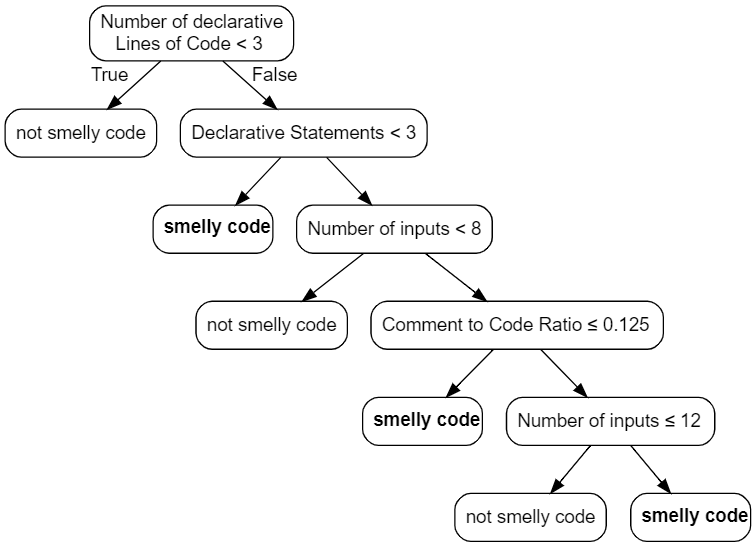
\includegraphics[width=400px]{figures/lpl_detection.png}
\caption{Decision tree model which indicates a Long Parameter List.}
\label{fig:lpl_detecion}
\end{figure}

\begin{table*}[t]
\centering
\begin{tabular}{lllllllllc}
\toprule
\textbf{Code smell} &   \textbf{Leaves}    & \textbf{Depth} & \textbf{TN} & \textbf{TP} & \textbf{FN} & \textbf{FP} & \textbf{Precision} & \textbf{Recall} & \textbf{F-measure} \\ 
\toprule
lpl & 6 & 5 & 106 & 29  & 9 & 6 & 0,841 & 0,856 & 0,849  \\
lm  & 6 & 3 & 462 & 137 & 4 & 2 & 0,973 & 0,976 & 0,972  \\
gc  & 3 & 2 & 47  & 14  & 2 & 2 & 0,843 & 0,889 & 0,878  \\
rb  & 3 & 2 & 84  & 27  & 9 & 5 & 0,750 & 0,724 & 0,721 \\
\bottomrule
\end{tabular}
\caption{Effectivity result}
\label{tbl:effectivityTable}
\end{table*}

\section{Study Procedure} \label{sec:studyProcedure}

%Based on the RQs (research questions), we aim to evaluate the following hypotheses: Providing the participant with the rules that predicts the code smell, through a graphical representation of the decision tree, \textbf{(H1)} we're going to have a better agreement among developers about the occurrence of a certain type of code smell, \textbf{(H2)} participants are going to have a better confidence about the occurrence of a code smell and \textbf{(H3)} participants are going to take less time to evaluate the occurrence of a code smell. 
The core procedure of our study is to test two distinctive treatments for different subjects (participants): evaluation of code smell with a decision tree visualization and evaluation of code smell without decision tree visualization. At the same time, we must assure the equivalence of evaluations from participants splitting several code snippets into two groups: in each group, each participant evaluates a task (a code snippet that hosts a code smell) along with a distinctive treatment.

From the previous paragraph, we may infer two independent variables with two levels each: two groups of tasks with two treatments each. Hence a 2 by 2 matrix-like design, or Latin Square design \cite{box2005statistics}, is suitable to accomplish our research needs. Figure \ref{fig:latinSquare} represents the experiment design applied to the present research and it is disposed as follows:
\begin{itemize}
    \item \textbf{Rows}: participants are shuffled in rows, namely participant 1 and participant 2;
    \item \textbf{Columns}: in the columns, there are 2 fixed groups of tasks, each task containing a source code (class or method) affected by a specific code smell type;
    \item \textbf{Cells}: treatment applied to some task, addressed to some participant. "DT" stands for "Decision Tree" - the decision tree model is available to be visualized - whereas "No DT" stands for "No Decision Tree" - the decision tree model visualization is omitted.
\end{itemize}

\begin{figure}[t]
\centering
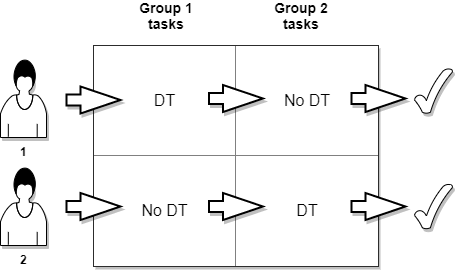
\includegraphics[width=300px]{figures/Latim_square_desing.png}
\caption{Experiment design. A 2x2 latin square.}
\label{fig:latinSquare}
\end{figure}

This experiment aims to collect the opinion of many participants about to what extent they (dis)agree about the existence of certain code smell type in selected code snippets. A user-friendly internet-based application was designed and suited to gather such opinions, having a business logic that complies with the experiment design showed in Figure \ref{fig:latinSquare}. The application is fully available at Github \footnote{\hyperlink{https://github.com/christianorossini/masterSurvey}{https://github.com/christianorossini/masterSurvey}}.

The application's URL was published on the Internet, mainly in social networks focused on IT professionals involved with Software Engineering, to invite potential participants.  After the invitation acceptance, the candidate finds the following flow, illustrated in Figure \ref{fig:experimentSteps}:

\begin{figure}[ht]
\centering
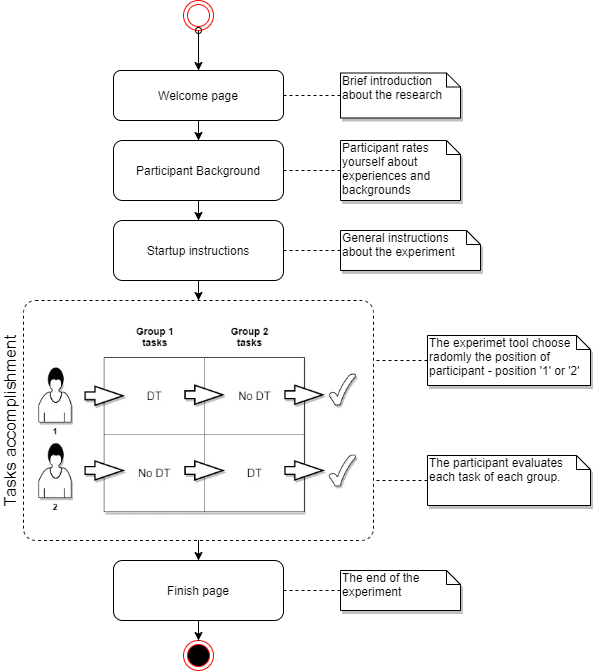
\includegraphics[width=13cm]{figures/experiment_flow.png}
\caption{Steps of the experiment}
\label{fig:experimentSteps}
\end{figure}

\begin{enumerate}
    \item \textit{Welcome page}: In the beginning, we present a welcome page to the participant with a brief description about the context of the study.
    
    \item \textit{Participant's background}: the participant rates its own experience about software development, object-oriented development, Java programming language, code revision and code smell detection. Each developer had to assign a rating which varies from "I do not have any experience" until "Very High".  Besides, the participant is asked about his highest academic degree so far, what's his origin (Industry, academy or both) and what is his experience in software development in years. The complete questionnaire can be found in the Appendix~\ref{appe:B}.
    
    \item \textit{Startup instructions}: at this stage, the experiment tool explains what is expected from the participant throughout the experiment. It includes how many tasks must be accomplished, what is the purpose of the tasks, what is the possible scenarios of code evaluation and a brief introduction about what is a decision tree. An example of a decision tree, as similar to those presented during experiment execution,  is shown to the participant in order to get familiarity with the metric-based rules. After clicking the button "Start experiment", the participant is forwarded to the tasks accomplishment step, where he starts to evaluate Java codes.  
    
    \item \textit{Tasks accomplishment}: at this point, the participants should accomplish a sequence of 12 tasks. This step is detailed in Section \ref{sec:tasksAccomplishment}.  
    
    \item \textit{Finish page}: once all tasks are accomplished, the experiment tool shows a page confirming that the experiment is ended.
    
\end{enumerate}

\section{Tasks accomplishment} \label{sec:tasksAccomplishment}

To our context, a task is an evaluation unit which has a correspondent Java code, chosen from a list of detected (predicted) smelly codes that are supposed to be affected by one of the code smells of Section \ref{sec:codeSmellTypes}. As we can observe in the experiment design illustrated in Figure \ref{fig:latinSquare}, the tasks are divided into two groups, each group with six tasks. Four of these tasks are control tasks or, as we call, "dummy" tasks. The dummy tasks aim to limit the biased \cite{palomba2014they} and carelessly participations, so we might filter participants that indicate the same answers without any criterion. Therefore, we have twelve tasks, but only eight are considered valid tasks (see Table \ref{tbl:tasksGroup1} and Table \ref{tbl:tasksGroup2}).

 In order to suits the experiment design (Figure \ref{fig:latinSquare}), the experiment tool logically groups the participants in pairs, so each participant is assigned randomly as Participant 1 (row 1) or Participant 2 (row 2). Therefore, for each pair of new participants who accept the invitation to participate in the experiment in chronological order, the system randomly assigns the first participant to complete the tasks as participant 1 or participant 2. Thereafter, the second participant will fill the space not occupied by the first. For example, let's assume that participant A starts the experiment and participant B starts later. If the participant A is assigned randomly to be the Participant 2, the next participant, when starting the experiment, will be the Participant 1.

Depending on the row that was chosen for the participant, first or second row of the Latin Square, Participant 1 or 2 respectively, it determines how they're going to accomplish each group of tasks, i. e., what is the sequence of treatment that will be applied for each group. The treatments come inside each cell of the experiment design, so each treatment appears only once in every row and every column (see Figure \ref{fig:latinSquare}). As a result, each participant performs both groups of tasks and has the opportunity to visualize the correspondent decision tree model only in one of the groups of tasks. Such tasks divided into groups favor the minimization of the learning effect because the treatments are completely isolated from each other.

\begin{table*}[t]
\centering
\begin{tabular}{clc} 
\toprule
\multicolumn{1}{l}{Task ID} & \multicolumn{1}{l}{Class or method} & \multicolumn{1}{l}{Code smell Type} \\ 
\midrule
\#11 & org.apache.nutch.tools.Benchmark.benchmark & lpl \\
\#7 & \begin{tabular}[c]{@{}l@{}}org.apache.qpid.ra.inflow.QpidActivationSpec\\org.apache.qpid.ra.ConnectionFactoryProperties\end{tabular} & rb \\
\#4 & org.apache.ivy.plugins.resolver.BasicResolver.getDependency & lm \\
\#3 & org.apache.tools.ant.DirectoryScanner & gc \\
\bottomrule
\end{tabular}
\caption{Classes or methods that belongs to tasks of group 1}
\label{tbl:tasksGroup1}

\begin{tabular}{clc} 
\toprule
\multicolumn{1}{l}{Task ID} & \multicolumn{1}{c}{Class or method} & \multicolumn{1}{l}{Code smell Type} \\ 
\midrule
\#12 & org.apache.hadoop.fs.ProxyFileSystem.create & lpl \\
\#5 & \begin{tabular}[c]{@{}l@{}}org.apache.qpid.ra.QpidRAStreamMessage\\org.apache.qpid.ra.QpidRAMessage\end{tabular} & rb \\
\#6 & org.apache.pig.impl.logicalLayer.optimizer.PushUpFilter.check & lm \\
\#8 & org.eclipse.jdt.internal.core.util.PublicScanner & gc \\
\bottomrule
\end{tabular}
\caption{Classes or methods that belongs to tasks of group 2}
\label{tbl:tasksGroup2}

\end{table*}

From this point to further work the treatments mentioned above we refer as scenarios: in one scenario the participant will have the opportunity to evaluate a Java code with the support of the rules provided by a visual representation of the predictor (decision tree) while in another the participant evaluates the code without any support. 

The Figures \ref{fig:taskEnvironmentNoDT} and \ref{fig:taskEnvironmentDT} exhibit the environments designed to task accomplishment and they represents the scenarios explained previously. In both cases, the experiment tool presents the name and description of the current code smell that is being evaluated. This description is based on an informal definition presented by Fowler \cite{fowler1999refactoring} as well as derived descriptions \cite{hozano2018you, palomba2014they}, so it's a starting point to the task evaluation.

\begin{figure*}[t]
\centering
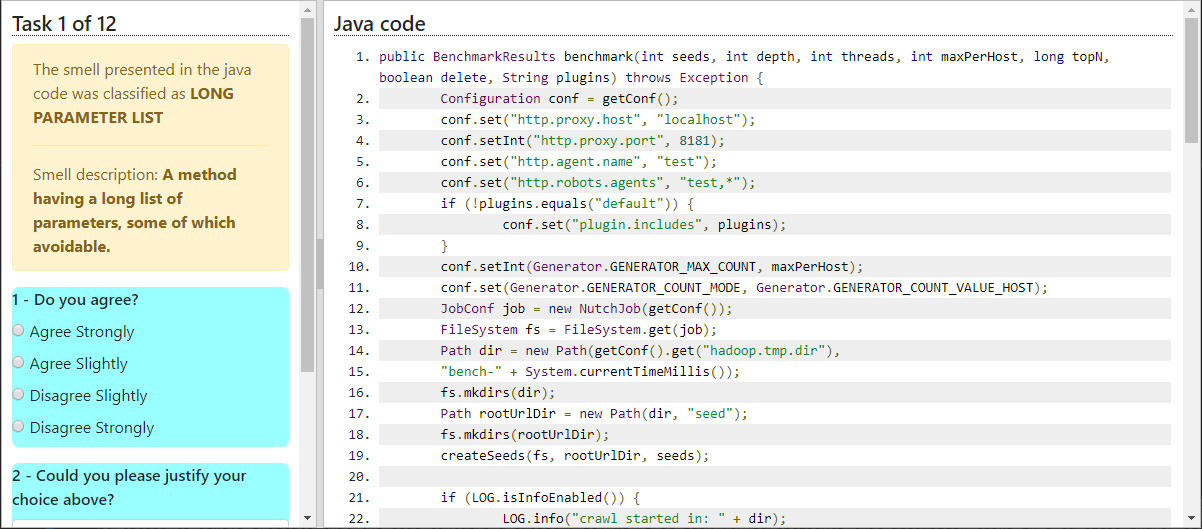
\includegraphics[width=400px]{figures/task_enviroment_noDT.PNG}
        \caption{Task environment without decision tree}
        \label{fig:taskEnvironmentNoDT}
\end{figure*}

\begin{figure*}[t]
\centering
        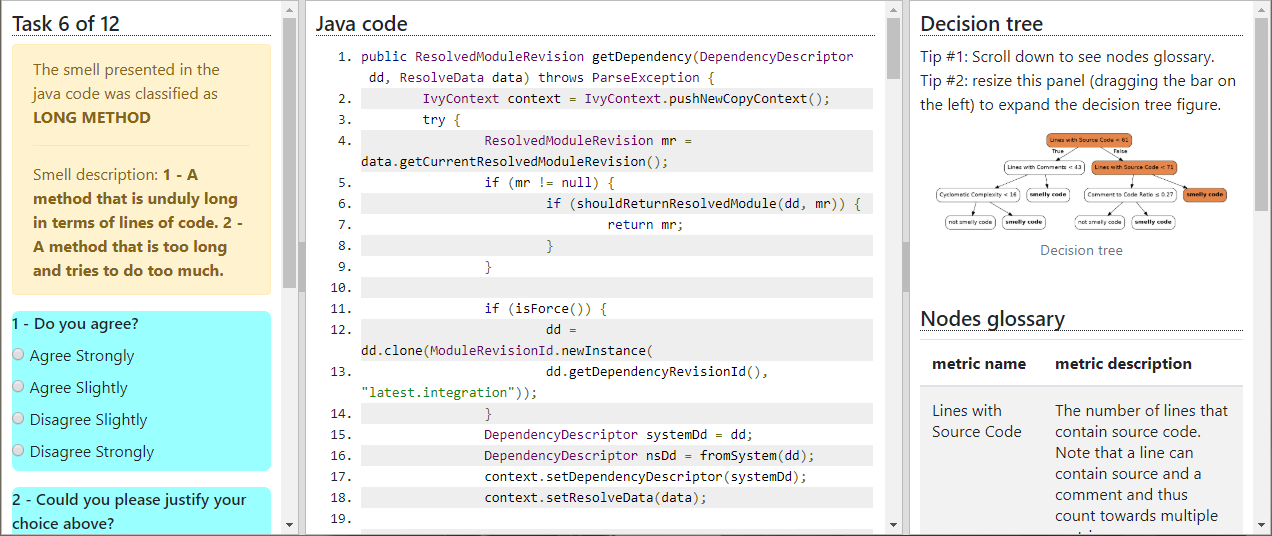
\includegraphics[width=400px]{figures/task_enviroment.PNG}
        \caption{Task environment with decision tree}
        \label{fig:taskEnvironmentDT}
    \end{figure*}  

For the scenario without decision tree visualization (Figure \ref{fig:taskEnvironmentNoDT}), the task environment has the following elements:
\begin{enumerate}
     \item \textbf{Task submission (left panel)}. For each task, the participant should submit a form composed of the following questions:\\
     \textit{1 - Do you agree?} - based on the code smell type described by the task, in this question the participants rates their degree of agreement regarding the smelliness of the Java code. Inspired by the Likert scale \cite{oppenheim2000questionnaire}, four options are available:
     \begin{itemize}
         \item Agree Strongly;
         \item Agree Slightly;
         \item Disagree Slightly;
         \item Disagree Strongly.
     \end{itemize}
     \textit{2 - Could you please justify your choice above?} - the participant should justify why he agrees or disagrees.
    \item \textbf{Java code (middle panel)}. The java code has to be evaluated by the participant in order to locate the suspicious code smell type described by the task.
\end{enumerate}

The scenario with decision tree visualization (Figure \ref{fig:taskEnvironmentDT}) has almost the same elements as the previous one, except by:
\begin{enumerate}
    \item \textbf{Task submission (left panel)}. Compared to the previous scenario, it has an extra question :    \\
     \textit{3 - What insights (contributions) did the decision tree give you in order to support your decision?} - to this question the participant should explain whether the decision tree model visualization contributes to reasoning about his evaluation.
    \item \textbf{Decision tree (right panel)}. The decision tree contains metric-based rules that lead to the code smell type that affects the java code presented by the task. It serves as a support for decision making. The highlighted path from the root node until leaf stands for the satisfied conditions within nodes that lead the predictor (machine learning classifier) to classify the current java code as smelly code (Figure \ref{fig:highlightedDT}). Additionally, the panel provides a sub-section called "Nodes Glossary" which contains a list of metrics and its descriptions aimed to facilitates the comprehension of the rules. 
\end{enumerate}

\begin{figure}[H]
\centering
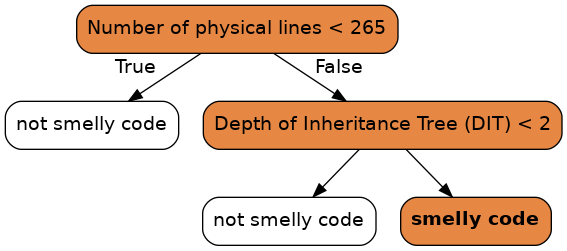
\includegraphics[width=300px]{figures/highlightedTree.png}
\caption{During a task evaluation, a highlighted path of a decision tree model is shown to the participant.}
\label{fig:highlightedDT}
\end{figure}
    
\section{Experiment execution and data inspection}

The experiment lasts about 4 weeks and had 30 participants who completed all the required tasks successfully. Afterward, we collected all the data from a relational database and we performed a data inspection to guarantee the quality of the data observed in the study. Thus, we analyzed the evaluations and open questions in order to identify problems that could interfere with the data analysis negatively.

As we mentioned in section \ref{sec:tasksAccomplishment}, we created "Dummy tasks" which are randomly selected java codes not affected by any of the code smells considered in our study. This was done to limit the bias \cite{palomba2014they} in the study, i.e., avoid that participants who always indicate that the code contains the suggested problem without reasoning about it. So, we first search for participants that accomplish tasks in a careless and/or biased way, analyzing how they performed tasks when faced with dummy tasks. For instance, we intentionally created a dummy task that defines and describes a god class. However, the associated java code has just a few lines of codes. Thus, we expected that the participant would mark "I strongly disagree" or, at minimum, "I Slightly disagree" in most of the dummy tasks presented to him. After data inspection, we noted that all of the participants not behave biased or carelessly. 

As mentioned previously, we obtained answers from 30 participants with different experiences in software development, Java programming language and code smell detection. The participant rated your personal experience that varies from "No experience" up to "Very High", distributed as illustrated in Figure \ref{fig:sefRatedExperience}. We note that the participants reported different experience levels (x-axis) and the great majority indicated experience higher or equal to "Low". For instance, the graph shows us that most of the participants have excellent skills in development, some of them having very high experience on it. It allows us to explore possibilities considering developers with different experience levels and with at least certain knowledge about the investigated context.

\begin{figure}[t]
\centering
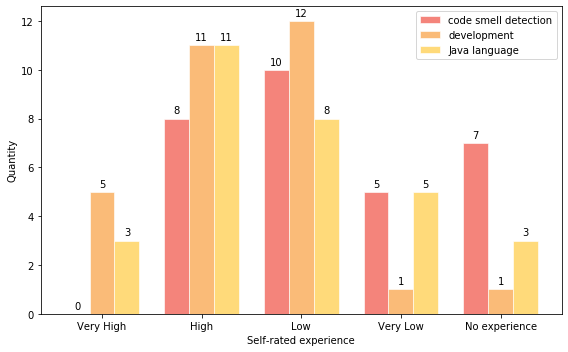
\includegraphics[scale=0.65]{figures/Self-rated_experience.png}
\caption{Self-rated experience from participants}
\label{fig:sefRatedExperience}
\end{figure}

\section{Data analysis}

After experiment execution and data collection we summarized the data to answer the research questions. We use methods to (i) analyze the inter-rater agreement among developers as well as developer's experiences and backgrounds that may influence such agreement, (ii) compute the confidence of evaluations considering the scenario with decision tree visualization and the scenario without decision tree and (iii) analyse the time spent by participants to accomplish each task considering both scenarios.

\subsection{Inter-rater agreement}

To answer the \textbf{RQ1}, we use a statistical method that calculates the inter-rater agreement among the developers’ evaluations. Fleiss Kappa \cite{fleiss1971measuring} measure the degree of agreement of the nominal or ordinal assessments made by multiple appraisers when assessing the same samples. Thus, this measure evaluates the concordance or agreement among multiple raters \cite{fleiss1971measuring}. This measure reports a number lower or equal to 1. If the Kappa value is equal to 1, then the raters are in complete agreement, unlike if the agreement is lower than 0 (zero), it means that there is no agreement among raters or it is weaker than expected by chance. Thus, we perform the following actions:
\begin{itemize}
    \item We collect the evaluations made for each group of tasks and split in two: evaluations aided by decision tree visualization and evaluations done without decision tree. Such evaluations produce a $4 \times N$ matrix, where 4 is the number of tasks from a group and \textit{N} is the number of raters (participants), as exemplified in Table \ref{tbl:participantsEvaluations}. The "Agrees" is obtained by evaluations marked as "Strong Agree" or "Slight Agree" as long as the evaluations assigned as "Strong Disagree" or "Slight Disagree" was computed as "Disagree". That convergence of two levels of "agree" or "disagree" in one was mandatory to calculate the Fleiss Kappa agreement properly. %Soon after, we sum all evaluations done per task, calculating the number of participants that agree with the code smell suggested by the task and the number of participants that disagree. 
    
\begin{table}[t]
\centering
\setlength{\extrarowheight}{0pt}
\addtolength{\extrarowheight}{\aboverulesep}
\addtolength{\extrarowheight}{\belowrulesep}
\setlength{\aboverulesep}{0pt}
\setlength{\belowrulesep}{0pt}
\begin{tabular}{c|rrrrrrrrrrrrrr} 
\toprule
\multirow{2}{*}{task} & \multicolumn{14}{c}{Participants} \\ 
\cmidrule{2-15}
 & 01 & 02 & 03 & 04 & 05 & 06 & 07 & 08 & 09 & 10 & 11 & 12 & 13 & 14 \\ 
\hline
\#3 & {\cellcolor[rgb]{0.502,0.502,0.502}} & {\cellcolor[rgb]{0.502,0.502,0.502}} & {\cellcolor[rgb]{0.502,0.502,0.502}} & {\cellcolor[rgb]{0.502,0.502,0.502}} & {\cellcolor[rgb]{0.502,0.502,0.502}} & {\cellcolor[rgb]{0.502,0.502,0.502}} & {\cellcolor[rgb]{0.502,0.502,0.502}} & {\cellcolor[rgb]{0.502,0.502,0.502}} & {\cellcolor[rgb]{0.502,0.502,0.502}} &  & {\cellcolor[rgb]{0.502,0.502,0.502}} & {\cellcolor[rgb]{0.502,0.502,0.502}} & {\cellcolor[rgb]{0.502,0.502,0.502}} & {\cellcolor[rgb]{0.502,0.502,0.502}} \\
\#4 &  & {\cellcolor[rgb]{0.502,0.502,0.502}} & {\cellcolor[rgb]{0.502,0.502,0.502}} & {\cellcolor[rgb]{0.502,0.502,0.502}} & {\cellcolor[rgb]{0.502,0.502,0.502}} & {\cellcolor[rgb]{0.502,0.502,0.502}} & {\cellcolor[rgb]{0.502,0.502,0.502}} & {\cellcolor[rgb]{0.502,0.502,0.502}} & {\cellcolor[rgb]{0.502,0.502,0.502}} & {\cellcolor[rgb]{0.502,0.502,0.502}} & {\cellcolor[rgb]{0.502,0.502,0.502}} & {\cellcolor[rgb]{0.502,0.502,0.502}} & {\cellcolor[rgb]{0.502,0.502,0.502}} & {\cellcolor[rgb]{0.502,0.502,0.502}} \\
\#11 & {\cellcolor[rgb]{0.502,0.502,0.502}} & {\cellcolor[rgb]{0.502,0.502,0.502}} & {\cellcolor[rgb]{0.502,0.502,0.502}} & {\cellcolor[rgb]{0.502,0.502,0.502}} & {\cellcolor[rgb]{0.502,0.502,0.502}} & {\cellcolor[rgb]{0.502,0.502,0.502}} & {\cellcolor[rgb]{0.502,0.502,0.502}} & {\cellcolor[rgb]{0.502,0.502,0.502}} & {\cellcolor[rgb]{0.502,0.502,0.502}} & {\cellcolor[rgb]{0.502,0.502,0.502}} & {\cellcolor[rgb]{0.502,0.502,0.502}} & {\cellcolor[rgb]{0.502,0.502,0.502}} & {\cellcolor[rgb]{0.502,0.502,0.502}} & {\cellcolor[rgb]{0.502,0.502,0.502}} \\
\#7 & {\cellcolor[rgb]{0.502,0.502,0.502}} & {\cellcolor[rgb]{0.502,0.502,0.502}} &  &  & {\cellcolor[rgb]{0.502,0.502,0.502}} &  &  & {\cellcolor[rgb]{0.502,0.502,0.502}} &  & {\cellcolor[rgb]{0.502,0.502,0.502}} & {\cellcolor[rgb]{0.502,0.502,0.502}} & {\cellcolor[rgb]{0.502,0.502,0.502}} & {\cellcolor[rgb]{0.502,0.502,0.502}} & {\cellcolor[rgb]{0.502,0.502,0.502}} \\
\bottomrule
\end{tabular}
\caption{Participants’ evaluations for tasks group 1, in DT scenario. The grey cell represents the 'Agree', the white is 'Disagree'.}
\label{tbl:participantsEvaluations}
\end{table}
    
    \item To each matrix of evaluations we compute the Fleiss’ Kappa measure in order to obtain the degree of agreement. As a result, we obtain 4 numeric values, each one representing the intersections (column $\times$ row) of the Latin Square design.
    
    \item We calculate the average of Kappa measures separated by scenario and compare.
\end{itemize}

%\subsubsection{Confidence of evaluations}

%In section \ref{sec:tasksAccomplishment} we mentioned that each developer evaluate the code smell based in four options. In two of them (strongly agree and slightly agree) he agrees, with different proportions though, that the source code hosts the code smell described in the tasks and in the other two options for the opposite. The level of confidence considers how much assignments of "slight" or "strong" the developers did. So we consider that a developer who evaluates a task as "Strongly agree" or "Strongly disagree" was made with more confidence than who evaluates a task as "Slightly agree" or "Slightly disagree". Thus, we converted all assignments of "Strong" as level of confidence 2 and assignments of "Slight" as level of confidence 1. 

\subsection{Time spent to accomplish tasks}

To answer the \textbf{R2}, we measure the time that the participant spend to
accomplish tasks with or without decision tree visualization, as a measurement of effort. During the experiment execution, all tasks were time-sensitive. It means that the experiment tool was designed with a time trigger that starts a time count whenever the participant explicitly starts a task and it stops when the participant submits such task. The time interval is stored in seconds and after converted in minutes to improve the readability.

\subsection{The usefulness of decision trees for decision making}

To answer the \textbf{RQ3}, we gathered all answers from the open question which asks the participant about what the insights/contributions were given by decision tree in order to support the decision making, considering the context of the task that is under evaluation. All the answers were analyzed by the authors and after we use the coding technique 
\cite{seaman1999qualitative} to categorize the detected contributions from qualitative data. From the analysis of the answers, we classified as good contributions to decision making the opinions which stated that the decision tree was useful for the presented evaluation context. 


